\documentclass[a4paper]{report}

% import packages
\usepackage{fancyhdr}
\usepackage{mwe}
\usepackage{amsmath}
\usepackage{setspace}
\usepackage{braket}
\usepackage{bm}
\usepackage{booktabs}
\usepackage{hyperref}
\usepackage[version = 4]{mhchem}

% import macros
% macros for math mode
\newcommand{\hamil}{\hat{\mathcal{H}}}
\newcommand{\kpsi}{\ket\Psi}
\newcommand{\dif}{\:\mathrm{d}}
\newcommand{\eps}{\epsilon}
\newcommand{\perturbE}[2][i]{% usage: \perturbE[subscript]{order}
E^{(#2)}_{#1}
}
\newcommand{\perturbPsi}[2][i]{% usage: \perturbPsi[subscript]{order}
\ket{\Psi_{#1}^{(#2)}}
}

% macros for text mode
\newcommand{\SE}{Schr{\"o}dinger equation}


% specify header and footers
\pagestyle{fancy}
\fancyhead{}
\fancyfoot{}
\renewcommand{\footrulewidth}{0.4pt}
\fancyhead[RO]{\textsl{\rightmark}}
\fancyfoot[LO]{\textsl{\leftmark}}
\fancyfoot[RO]{\thepage}

% bibliography
\usepackage[backend = bibtex, sorting = none]{biblatex} \addbibresource{bib.bib}

\begin{document}

\pagenumbering{roman}

\begin{titlepage}
\begin{center}
{ \Large
	\uppercase{Investigations into Molecular Dimers via Monte Carlo Many-Body Methods}

	\vspace{3 cm}

	\uppercase{BY \\ DAVID QIU}

	\vspace{3 cm}

	{\Large UNDERGRADUATE THESIS}

	\vspace{1 cm}

	{\large Submitted to the Department of Chemistry in the College of
	Liberal Arts and Sciences as part of an undergraduate research program.}

	\vspace{1 cm}

	{\large University of Illinois at Urbana-Champaign, 2020}

	\vspace{1 cm}

	{\large Urbana, Illinois}

}
\end{center}

\vfill

\begin{flushleft}

	{\large Faculty Advisors: \\
	DR.\ SO HIRATA, PROFESSOR OF CHEMISTRY \\
	DR.\ ALEXANDER DORAN, POSTDOCTORAL SCHOLAR}

\end{flushleft}
\end{titlepage}


\tableofcontents

\chapter*{Abstract}
\addcontentsline{toc}{chapter}{Abstract}

abstract goes here

\newpage

\pagenumbering{arabic}

\doublespacing

% INTRODUCTION
\chapter{Introduction}

This chapter aims to introduce the reader to the basic mathematical and
quantum-mechanical topics needed to achieve a full understanding of the topics
presented in this thesis. This chapter borrows heavily from the textbook written
by Szabo and Ostlund, and material discussed in this chapter cites it as a
reference unless otherwise noted. \cite{szabo}

Section \ref{s:math} introduces the mathematical concepts and conventions used
throughout the text. It assumes at the very least a basic knowledge of
multivariable calculus, applied linear algebra, and the quantum mechanics
encountered in an introductory semester of physical chemistry. Section
\ref{s:problem} posits the many-body electronic problem, the central subject of
computational chemistry. Section \ref{s:hf} describes the Hartree-Fock
approximation, arguably the most important first approximation to solutions of
the many-body electronic problem. Sections \ref{s:post-hf} and \ref{s:pt} then
describe post-Hartree-Fock methods, which expand upon and refine the
Hartree-Fock approximation to provide more accurate results. In particular,
perturbation theory is discussed in greater detail due to its relevance to the
subject of this thesis, the MC-MP2 method.

\section{Mathematical Review}
\label{s:math}

\subsection{Dirac Notation}

Throughout the field of quantum mechanics, \emph{Dirac's bra-ket notation} is
widely used to express complex functions and their corresponding inner products,
and greatly lessens the burden associated with their notation. It also elegantly
encapsules the relationship between functions and vectors.

Any single-valued, continuous, square-integrable function $a(x)$ on some complex
interval can be described as a vector lying in \emph{Hilbert space}, an abstract
inner product space that extends the concept of Euclidean space to an infinite
number of dimensions. The intuition behind this one-to-one correspondence
between certain functions and infinite-dimensional vectors is best left to its
own section (see Appendix TBD).

$a(x)$ is represented as a \emph{ket} vector living in a Hilbert space termed
ket space, and is denoted as follows.

\begin{equation}
	a(x) \equiv \ket{a}
\end{equation}

Its complex conjugate, $a(x)^*$, is represented as a \emph{bra} vector living in
the dual (or, more descriptively, adjoint) space of ket space, and is denoted as

\begin{equation}
	a(x)^* \equiv \bra{a} = \ket{a}^\dagger,
\end{equation}

\noindent where the dagger denotes the adjoint. Observe that the inner product
between any two functions $a(x)$, $b(x)$ then becomes

\begin{equation}
	\int a(x)^* b(x) \dif x = \int \bra{a} \ket{b} \dif x \equiv \braket{a|b},
\end{equation}

\noindent which is exactly analogous to the definition of an inner product for
vectors.

\subsection{Atomic Units}

Atomic units arise from dropping the mathematical constants (e.g.\ $h$, $\pi$,
etc.) in each term of the \SE. For instance, the \SE\ of atomic hydrogen,

\begin{equation}
	\left(
	- \frac{\hbar^2}{2 m_e} \nabla^2
	- \frac{e^2}{4 \pi \eps_0 r}
	\right)
	\Psi = E \Psi,
\end{equation}

\noindent reduces to the form

\begin{equation}
	\left(
	- \frac{1}{2} \nabla^2
	- \frac{1}{r}
	\right)
	\Psi = E \Psi
\end{equation}

\noindent in atomic units. A brief summary of atomic units and their conversion
factors has been tabulated in Table \ref{t:atomic} for the reader's convenience.
All subsequent equations hereafter will be derived in terms of these atomic
units.

\begin{table}[]
\begin{tabular}{@{}lll@{}}
\toprule
Physical quantity & Atomic unit               & Value in SI units                                           \\ \midrule
Length            & Bohr radius               & $a_0 = 5.291772 \times 10^{-11}$ m                       \\
Mass              & Electron mass             & $m_e = 9.109383 \times 10^{-31}$ kg                      \\
Charge            & Electron charge           & $e = 1.602176 \times 10^{-19}$ C                         \\
Energy            & Hartree                   & $\frac{\hbar^2}{m_e a_0^2} = 4.359744 \times 10^{-18}$ J \\
Momentum          & Reduced Planck's constant & $\hbar = 1.054571817 \times 10^{-34}$ J $\cdot$ s           \\ \bottomrule
\end{tabular}
\caption{Table of atomic units and their conversion to SI units.}
\label{t:atomic}
\end{table}


\subsection{Electronic Orbitals}

This thesis will be primarily concerned with \emph{electronic} wavefunctions
describing the dynamics of the electrons in a molecular system, rather than
considering the total wavefunction describing the nuclei. The reasoning for
doing so is outlined in Section \ref{s:problem}.

The electronic wavefunction for a single electron is defined as a \emph{spatial
orbital}, and is denoted by $\psi(\bm r)$, where $\bm r$ represents a vector
containing the $x, y, z$ spatial coordinates of the electron. The spatial
orbital fully defines the spatial distribution of a single electron. We
furthermore define the \emph{spin orbital} $\chi(\bm x)$ as

\begin{equation}
	\chi_{j}(\bm x) =
	\begin{cases}
		\psi_{i}(\bm r) \alpha(\omega)  & \text{if } j = 2i - 1, \\
		\psi_{i}(\bm r) \beta(\omega)   & \text{if } j = 2i, \\
	\end{cases}
	\label{eq:spino}
\end{equation}

\noindent where $\bm x$ is a four-vector containing the three spatial
coordinates (i.e.\ the components of $\bm r$) and the additional spin coordinate
$\omega$. Here, $\alpha(\omega), \beta(\omega)$ are any two arbitrary orthogonal
functions of some arbitrary spin coordinate $\omega$, and represent the electron
having $m_s = \pm \frac{1}{2}$ respectively. Thus, the spin orbital also
distinguishes between electrons that may have the same spatial distribution, but
have different spins. An example of this is the singlet ground state of
molecular hydrogen, where the electrons occupy the same spatial 1s molecular
orbital (MO), but have opposing spins.  Thus, the two electrons are said to
occupy separate spin orbitals.

It is now worth mentioning the conventions for indexing the spatial and spin
orbitals. Typically, the number of electrons in a system is represented by $N$,
while the total number of possible spatial orbitals (not just the occupied ones)
is given by $K$, where $K \geq \frac{N}{2}$. Thus, the total number of spin orbitals is
given by $2K$, directly following from equation \ref{eq:spino}. This convention
will be followed throughout the rest of this thesis.

\subsection{Hartree Products}

The full Hamiltonian of a molecular system includes two-body interactions that
complicate derivation of the solutions. However, if the Hamiltonian can be
approximated as a series of one-electron interactions, e.g.

\begin{equation}
	\hamil \approx \sum_i^N \hat h(\bm r_i) ,
	\label{eq:onehamil}
\end{equation}

\noindent where $\hat h(\bm r_i)$ is a one-electron Hamiltonian that
\emph{approximates} the contribution of the $i$th electron to the total energy,
e.g.\ by somehow averaging the contribution of other electrons out (c.f. Section
\ref{s:hf}).

Given this approximation, if the series of one-electron Hamiltonians is solved
for all $i$, and the spin orbitals $\{ \chi_j \}$ are known to satisfy the
relation

\begin{equation}
	\hat h(\bm r_i) \chi_j (\bm x_i) = \epsilon_j \chi_j(\bm x_i),
\end{equation}

\noindent then it can be shown that the corresponding \emph{approximate} total
electronic wavefunction $\Psi$, the eigenfunction satisfying equation
\ref{eq:onehamil}, is given by the \emph{Hartree product}

\begin{equation}
	\Psi(\bm x_1, \bm x_2, \dots, \bm x_N) = \chi_i(\bm x_1) \chi_j(\bm x_2) \dots \chi_k(\bm x_N),
	\label{eq:hartree}
\end{equation}

\noindent with a corresponding eigenvalue

\begin{equation}
	E = \eps_i + \eps_j + \cdots + \eps_k.
\end{equation}

Note that the Hartree product approximates any possible state of the molecular
system, not just the ground state, hence the unusual indexing of the spin
orbitals in equation \ref{eq:hartree}. $i, j, k$ need not satisfy any relation
other than that they are distinct and less than or equal to $2K$, and thus the
Hartree product can represent the either the ground state or any arbitrary
excited state. This makes Hartree products useful first approximations to the
true nature of the total electronic wavefunction.

\subsection{Slater Determinants}

However, even forgiving the fact that the Hartree product is an approximation to
the total electronic wavefunction, there exists a fundamental failure of the
Hartree product in its ability to describe real quantum systems.  Namely, it
does not treat electrons as fermions, which necessarily satisfy the Pauli
exclusion principle. The Pauli exclusion principle in turn requires that all
electronic wavefunctions must be antisymmetric with respect to exchange, i.e.

\begin{multline}
	\Psi(\bm x_1, \bm x_2, \dots, \bm x_i, \dots, \bm x_j, \dots, \bm x_N) \\
	= - \Psi(\bm x_1, \bm x_2, \dots, \bm x_j, \dots, \bm x_i, \dots, \bm x_N).
\end{multline}

Because of the commutativity of simple multiplication, the Hartree product does
not satisfy this relation, and thus is not a satisfactory description of the
electronic wavefunction. Instead, there must exist a more complex relationship
between the total electronic wavefunction and the one-electron spin orbitals
satisfying equation \ref{eq:onehamil}. One method of antisymmetrizing the total
electronic wavefunction is to represent it as a normalized determinant of a
matrix of spin orbitals, where the $i$th row and $j$th column contain the spin
orbital $\chi_j(\bm x_i)$, i.e.

\begin{equation}
	\Psi(\bm x_1, \bm x_2, \dots, \bm x_N)
	=
	\frac{1}{\sqrt{N!}}
	\begin{vmatrix}
		\chi_i (\bm x_1) & \chi_j (\bm x_1) & \cdots & \chi_k (\bm x_1) \\
		\chi_i (\bm x_2) & \chi_j (\bm x_2) & \cdots & \chi_k (\bm x_2) \\
		\vdots & \vdots & \ddots & \vdots \\
		\chi_i (\bm x_N) & \chi_j (\bm x_N) & \cdots & \chi_k (\bm x_N)
	\end{vmatrix}
	.
	\label{eq:slater}
\end{equation}

Equation \ref{eq:slater} defines the \emph{Slater determinant}, and is the
antisymmetrized total electronic wavefunction of a $N$-electron system. The
antisymmetry property of the Slater determinant can be verified by noting that
the interchange of any two electrons is equivalent to interchanging two rows in
the determinant. The interchange of any two rows or columns of a determinant
reverses the sign. This is made especially apparent in the \emph{Leibniz formula
for determinants},

\begin{equation}
	|A| = \sum_{\sigma \in S_n} \text{sgn}(\sigma) \prod^n_i A_{\sigma(i), i},
\end{equation}

\noindent where $\sigma$ is an arbitrary permutation in the set of all $n!$
possible permutations $S_n$, and $\text{sgn}(\sigma)$ is the signature of the
permutation, which is equal to unity and reverses sign following each single
interchange of indices.

\section{The Many-body Electronic Problem}
\label{s:problem}

Given the mathematical review in the preceding section, one is now in a position
to discuss the many-body electronic problem and the computational difficulty
involved in its solution. The central interest of electronic structure theory is
the determination of solutions to the non-relativistic, time-independent \SE

\begin{equation}
	\hamil \ket{\Psi(\{\bm{r_i}\} , \{\bm{R_I}\}} = E \kpsi
\label{eq:tise}
\end{equation}

\noindent where $\kpsi$ is an exact wavefunction for the molecular system,
describing both the nuclei and electrons simultaneously, and $E$ is the
corresponding energy of $\kpsi$. The Hamiltonian is in turn given by the
relation

\begin{equation}
	\hamil = - \sum_i^n \frac{1}{2}\nabla_i^2
	- \sum_I^N \frac{1}{2}\nabla_I^2
	 - \sum_i^n \sum_I^N \frac{Z_I}{r_{iI}}
	 + \sum_i^n \sum_{j > i}^n \frac{1}{r_{ij}}
	 + \sum_I^N \sum_{J > I}^N \frac{Z_I Z_J}{r_{AB}}.
\label{eq:fullh}
\end{equation}

Here, lowercase indices index over the $n$ electrons, while uppercase indices
index over the $N$ nuclei. $Z_I$ represents the charge of a given nucleus $I$,
and $r$ has the usual definition of being the distance between any two pairs of
coordinates. A closer observation reveals the intuition summarized in the above
equation. The first and second terms denote the kinetic energy of the electrons
and nuclei respectively, while the third, fourth, and fifth terms denote Coulomb
attraction and repulsion within the molecular system.

As written above, equation \ref{eq:tise} is an extraordinarily involved $3(n +
N)$-dimensional non-linear partial differential equation (PDE), with no
analytical solution known for molecular systems larger than hydrogen.
Furthermore, the eigenvalues and eigenfunctions of equation \ref{eq:tise} are
seldom desired. Nuclear coordinates are typically already known via experimental
techniques such as X-ray diffraction. The computational chemist wishes to
determine purely the electronic component of the wavefunction and its
corresponding eigenvalues, both of which collectively govern pertinent chemical
properties such as polarizability, polarity, reactivity, and optical spectra.

Thus, further approximations must be made to simplify equations \ref{eq:tise}
and \ref{eq:fullh} and isolate the many-body electronic problem.

\subsection{Non-relativistic Approximation}

It is worth mentioning that the written form of \ref{eq:fullh} already
encompasses the non-relativistic approximation, which neglects special
relativistic effects electrons experience with sufficiently high linear and
angular momenta \cite{rel1, rel2}. While this effect is especially significant
for heavy atoms such as transition and post-transition metals (see the seminal
reviews of Pyykk{\"o} and coworkers \cite{pyykko1, pyykko2, pyykko3}), it
typically results in little error for organic systems such as those investigated
hereonafter, and thus can be neglected.

\subsection{Born-Oppenheimer Approximation}

Nuclei are orders of magnitude more massive than electrons, and thus experience
different time scales of motion, i.e.\ nuclei move far more slowly than
electrons given the same momentum. In the context of the many-body electronic
problem, this implies that nuclei can be essentially regarded as fixed points in
space, and can be treated as given parameters to the problem. In other words,
the problem is said to depend on the nuclear coordinates \emph{parametrically}
rather than explicitly. This does not imply that electron-nuclei interactions
neglected, but rather that the interactions are \emph{de-coupled} from one
another, and that one-body nuclear interactions treated as constants and
two-body electron-nuclei interactions are treated as one-body interactions.

Thus, the nuclear terms (the second and fifth terms of equation \ref{eq:fullh})
can be dropped and treated as added constants to the final energy of the
molecular state. These dropped nuclear terms include the translational,
vibrational, and rotational energies of the molecule. Equations \ref{eq:tise}
and \ref{eq:fullh} reduce to

\begin{equation}
	\hamil \ket{\Psi(\{\bm{r_i}\} ; \{\bm{R_I}\}} = E \kpsi,
\label{eq:BO}
\end{equation}

\noindent where $\kpsi$, $E$ now represent the \emph{electronic} wavefunction
and its corresponding energy, and

\begin{equation}
\hamil = - \sum_i^n \frac{1}{2} \nabla_i^2
	 - \sum_i^n \sum_I^N \frac{Z_I}{r_{iI}}
	 + \sum_i^n \sum_{j > i}^n \frac{1}{r_{ij}}.
\label{eq:BOhamil}
\end{equation}

\subsection{Statement of the Problem}

The many-body electronic problem is summarized in equations \ref{eq:BO} and
\ref{eq:BOhamil}, and can be made explicit as follows: \emph{given a set of
nuclear coordinates $\{ R_I \}$, what are the corresponding wavefunctions and
energies which satisfy the electronic \SE ?}

No general method has been devised to directly solve the many-body electronic
problem. Even with the drastic simplification conferred by the non-relativistic
approximation, and the $3N$ fewer degrees of freedom resulting from the
Born-Oppenheimer approximation, equation \ref{eq:BO} remains a $3n$-dimensional
non-linear PDE with no analytical solution. The subsequent sections in this
chapter detail further approximations one can make to arrive at numerical
solutions to the many-body electronic problem.

\section{The Hartree-Fock Approximation}
\label{s:hf}

\subsection{Physicists' Notation}

Prior to further discussion, it is worth mentioning a notational shorthand for
one-electron and two-electron Coulomb integrals that are so commonly encountered
in further derivation of Hartree-Fock methods. This notation is known as
\emph{physicists' notation}. For the one-electron case,

\begin{equation}
	\braket{a|h|b} = \int \chi_a^* (\bm x_i) h(\bm r_i) \chi_b (\bm x_i) \dif x_i,
\end{equation}

\noindent and for the two-electron case,

\begin{equation}
	\braket{ab|cd} = \iint \chi_a^* (\bm x_i) \chi_b^*(\bm x_j)
	\frac{1}{r_{ij}}
	\chi_c (\bm x_i) \chi_d (\bm x_j) \dif \bm x_i \dif \bm x_j.
\end{equation}

It is implied that during integration, spin orbitals lying left of the central
separator are transformed to their corresponding complex conjugates, and are
functions of $\bm x_i, \bm x_j$ respectively. Spin orbitals lying to the right
are similarly defined, but are left unaffected during integration.

One can furthermore define the \emph{anti-symmetrized} two-electron Coulomb
integration in physicists' notation through the addition of an additional
vertical separator as follows.

\begin{equation}
	\bra{ab} \ket{cd} = \braket{ab|cd} - \braket{ab|dc}.
\end{equation}

\subsection{The Hartree-Fock Equations}

The most troublesome aspect of the many-body electronic problem is the two-body
Coulomb interaction which makes it inseparable. However, to approximate the
two-body Coulomb interaction that a single electron experiences, one could
compute an average potential generated from all other electrons, thus
simplifying the many-body electronic problem.

The \emph{Hartree-Fock (HF) approximation} achieves this by decomposing the
N-electron \SE\ detailed in equations \ref{eq:BO} and \ref{eq:BOhamil} into $N$
one-electron \emph{Hartree-Fock equations}, which satisfy the relation

\begin{equation}
\begin{split}
	\label{eq:fock}
	\hat f(\bm x_i) \chi_a (\bm x_i)
	&= \hat h(\bm x_i) \chi_a (\bm x_i) \\
	&\quad + \sum_{b \neq a}^{2K} \left[ \int |\chi_b(\bm x_j)|^2 \frac{1}{r_{ij}} \dif \bm x_j \right] \chi_a (\bm x_i) \\
	&\quad - \sum_{b \neq a}^{2K} \left[ \int \chi_b^*(\bm x_j) \chi_a(\bm x_j) \frac{1}{r_{ij}} \dif \bm x_j \right] \chi_b (\bm x_i) \\
	&= \eps_a \chi_a (\bm x_i)
\end{split}
\end{equation}

\noindent for all occupied spin orbitals, where $\hat f(\bm x_i)$ is termed the
\emph{Fock operator}, $\eps_a$ is the energy of the spin orbital $\chi_a$
occupied by electron $i$, $K$ is the number of given spatial basis functions,
and $\hat h (\bm x_i)$ is the simplified one-electron Hamiltonian

\begin{equation}
\hat h (\bm x_i) = - \frac{1}{2} \nabla_i^2
	           - \sum_I^M \frac{Z_I}{r_{iI}},
\end{equation}

\noindent given $M$ nuclei.

The seemingly complicated integro-differential Hartree-Fock equations in
equation \ref{eq:fock} can be decomposed term-by-term to assess the intuition
behind the expression. The bracketed quantity in the second term can be
interpreted as a \emph{mean-field Coulomb operator}, which computes the average
potential by the $i$th electron generated by an electron occupying the $b$th
spin orbital. This can be made explicit in the expression

\begin{equation}
\hat J_b (\bm x_i) = \int |\chi_b (\bm x_j)|^2 \frac{1}{r_{ij}} \dif \bm x_j.
\end{equation}

The third term in equation \ref{eq:fock} can also be written in terms of a new
operator known as the \emph{exchange operator}, though this does not have a
simple classical interpretation as did the mean-field Coulomb operator, and
arises purely from the antisymmetric nature of the wavefunction as expressed by
the Slater determinant. The action of the exchange operator on a spin orbital is
given by the equation

\begin{equation}
	\hat K_b (\bm x_i) \chi_a(\bm x_i) =
	\left[ \int \chi_b^* (\bm x_j) \frac{1}{r_{ij}} \chi_a(\bm x_j) \dif \bm x_j \right]
	\chi_b (\bm x_i).
\end{equation}

An ad-hoc justification for the presence of this term in the Hartree-Fock
equations is to account for the lower energy of systems of parallel spins, a
quantum-mechanical phenomenon known as \emph{exchange correlation}. This process
can be rationalized by noting that electrons with parallel spins have an
inherently lower probability of being near each other because of Pauli
exclusion, and thus experience less classical Coulomb repulsion between one
another, lowering the energy of the system.

Given the Coulomb and exchange operators, the Hartree-Fock equations can be
re-written as

\begin{equation}
\hat f(\bm x_i) \chi_a (\bm x_i) =
\left[ h(\bm x_i)
+ \sum_{b \neq a}^{2K} \hat J_b (\bm x_i)
- \sum_{b \neq a}^{2K} \hat K_b (\bm x_i) \right] \chi_a (\bm x_i)
= \eps_a \chi_a(\bm x_i).
\label{eq:hf}
\end{equation}

\subsection{The Self-Consistent Field Method}

The Hartree-Fock equations expressed in equation \ref{eq:hf} still present with
immense computational difficulty, in that the Fock operator depends on the
eigenfunctions themselves. Thus, the Hartree-Fock equations are
\emph{pseudo-eigenvalue problems}, as the operator itself depends on the
solutions obtained from the operator, and can only be solved iteratively.
Nevertheless, there at least exists a clear method for solving this problem,
dubbed the \emph{self-consistent field method} (SCF method). The general
theoretical procedure is as follows.

\begin{enumerate}

	\item Assuming one has already been given a molecule (i.e.\ the set of
		nuclear coordinates, atomic numbers, and number of electrons),
		one must provide a basis set of spatial \emph{atomic orbitals}
		(AOs). Many different basis sets are available in the literature
		for varying applications, and it is to the chemists' discretion
		which to use.

	\item Generate the Fock operator using the given basis set.

	\item The generated Fock operator to solve for the new eigenvalues and
		new eigenvectors, which are closer approximations to the true
		eigenvalues and eigenvectors of the Fock operator. The new
		eigenvectors are linear combinations of the AOs, and are termed
		\emph{molecular orbitals} (MOs).

	\item Repeat steps 2 and 3 until the eigenvalues and eigenvectors reach
		sufficient convergence.

\end{enumerate}

Ideally, this provides a set of MOs defined in terms of the AO basis, with a
corresponding set of eigenvalues. Of course, this by no means provides a
practical implementation of the HF method. In practice, implementation of the HF
method is complicated by issues such as non-orthogonal basis functions, and
requires inclusion of more sophisticated techniques in numerical linear algebra
such as diagonalization and unitary transformations. This work will not discuss
such techniques, as its primary intent is to illustrate developments in MC-MP2
theory, and will treat obtained HF energies and orbitals as givens.
Nevertheless, MP2 builds off of the theoretical foundations laid out by the HF
method, and it is instructive to learn the fundamentals of the HF method as to
improve upon its results via MP2 theory.

% \subsection{The Hartree-Fock Energy}
%
% Assuming that the SCF method obtained the set of eigenvalues and eigenfunctions
% of the Fock operator, it is then sufficient to use these to obtain the
% \emph{Hartree-Fock energy}.

\section{Post-Hartree-Fock Methods}
\label{s:post-hf}

\emph{Post-Hartree-Fock methods} are computational methods aimed at achieving
more accurate solutions to the many-body electronic problem than those obtained
via the HF method. Each of these methods corrects for one (of multiple)
approximations made during solution of the HF equations. One such method,
second-order many-body perturbation theory (MP2), is the central topic of this
thesis, and is discussed in its own subsequent section. This section aims at
discussing alternative post-Hartree-Fock methods and their various shortcomings
as motivations for further development of MP2 theory.

\subsection{Configuration Interaction}

In the HF method, the ground state $N$-electron total electronic wavefunction is
evaluated as the Slater determinant of $N$ single-electron eigenfunctions of the
Fock operator. This incomplete, approximate representation of the total
electronic wavefunction necessarily over-estimates the ground state energy, per
the variational principle.

To achieve a finer upper bound to the ground state energy, one can include
contributions from other Slater determinants formed from the $N$ electrons all
$2K$ spin orbitals, not just those lowest in in energy. This requires the
computation of

\begin{equation}
	\binom{2K}{N} = \frac{2K!}{N!(2K - N)!}
\end{equation}

\noindent Slater determinants. Thus, the \emph{method of configuration
interaction (CI)} aims at solving the variational problem

\begin{equation}
	\Psi = c_o \ket{\Psi_0} +  \sum_{a} \sum_{r} c_a^r \ket{\Psi_a^r}
	+ \sum_{a} \sum_{b > a} \sum_{r} \sum_{r > s} c_{ab}^{rs} \ket{\Psi_{ab}^{rs}}
	+ \cdots,
\label{eq:full-ci}
\end{equation}

\noindent with the second term representing a summation over all singly-excited
Slater determinants, the third term representing a summation over all
doubly-excited Slater determinants, and so on. Needless to say, solution of this
variational problem for all possible Slater determinants (full CI) is
extraordinarily computationally complex as the number of Slater determinants
required grows on the order of $2K!$. A full CI calculation of just molecular
nitrogen using the ANO basis (4s3p1d) requires $9.68 \times 10^9$ Slater
determinants. \cite{n2-ci}

With full CI being prohibitively expensive, an alternative is to truncate the
above variational problem past the doubly-excited Slater determinants in
equation \ref{eq:full-ci}, in a procedure known as singly and doubly excited CI
(SDCI). Alternatively, one can choose to vary the spin orbitals within the
Slater determinant simultaneously while varying the set of coefficients to
counteract the error introduced via truncation, in a procedure known as
multiconfiguration self-consistent-field (MCSCF).

However, truncated CI also suffers from a serious failure in that it fails to be
\emph{size-consistent}, i.e. its energy fails to scale with $N$ given $N$
interacting systems. In fact, its variational estimate of the energy tends
towards zero in the limit $N \rightarrow \infty$. For investigations into
molecular dimers (such as the ones discussed in this thesis) or larger systems
such as crystals, this shortcoming is fatal.  An investigation of why this is
true in the general case of truncated CI is rather involved and well beyond the
scope of this text.  Nevertheless, a brief mention of this shortcoming, in
conjunction with the computational cost of CI methods in general, is enough to
rationalize the relative scarcity of CI methods in computational chemistry
today.

\subsection{Pair and Coupled Pair Theories}

Pair and coupled pair theories are a broad family of methods that essentially
provide size-consistent approximations to the full CI method. This includes the
independent electron pair approximation (IEPA) and the coupled cluster (CC)
method. Of these theories, the CC method is the most competitive. A specific
instance of the CC method, CCSD(T) (coupled cluster single double triple)
provides some of the most highly accurate results available in computational
chemistry. \cite{cc1, cc2, cc3, cc4}

Thus, CC methods serve as a competitive benchmark for correlation energies
obtained using the MC-MP2 method discussed in this thesis. However, its
computational cost scaling makes it prohibitively expensive for very large
systems. Thus, further development of post-Hartree-Fock methods are still needed
to analyze very large molecular systems.

\section{Perturbation Theory}
\label{s:pt}

Perturbation theory is a theory encompassing a broad range of methods in
computational physics and chemistry aimed at improving approximations to complex
systems by constructing the application of successive refinements known as to
the eigenvalues and eigenfunctions of the approximate system. Here, the two most
pertinent examples to the many-body electronic structure problem are discussed.

\subsection{Rayleigh-Schr{\"o}dinger Perturbation Theory}

Suppose one is already given the eigenfunctions and eigenvalues of an
\emph{approximate} Hamiltonian $\hamil_0$, which relates to the full Hamiltonian
$\hamil$ through the addition of \emph{perturbation} $\hat V$, i.e.

\begin{equation}
	\hamil\ket{\Psi_i} = (\hamil_0 + \lambda\hat V) \ket{\Psi_i} = E_i \ket{\Psi_i}
	\label{eq:pt}
\end{equation}

\noindent where $\lambda$ is equal to unity, and used purely to keep track of
terms for future derivation. Next, let the eigenfunctions and eigenvalues of
$\hamil$ be expanded into a power series relation with respect to its
approximated counterparts.

\begin{align}
	\label{eq:e-pt}
	E_i &= E^{(0)}_i + \lambda E^{(1)}_i + \lambda^2 E^{(2)}_i + \cdots \\
	\label{eq:psi-pt}
	\ket{\Psi_i} &= \ket{\Psi^{(0)}_i} + \lambda \ket{\Psi^{(1)}_i} + \lambda^2 \ket{\Psi^{(2)}_i} + \cdots
\end{align}

\noindent where the superscripts represent the successively finer corrections to
the energy and wavefunction. For instance, $E_i^{(2)}$ represents the
second-order correction to the $i$th energy. This expansion of the eigenvalues
and eigenfunctions into a sum of successive corrections to their zeroth-order
approximations is \emph{Rayleigh-Schr{\"o}dinger perturbation theory} (RSPT). To
simplify this discussion, the expressions for third and higher-order
perturbations will not be discussed, for their expressions are exceedingly
cumbersome, and serve little purpose in the discussion of the MC-MP2 method, a
variant of second-order perturbation theory.

Next, let equations \ref{eq:e-pt} and \ref{eq:psi-pt} be substituted into the
perturbation expansion \ref{eq:pt}. Gathering the zeroth, first, and second
order terms corresponding to $1, \lambda, \lambda^2$ respectively, one finds

\begin{align}
	\hamil_0 \perturbPsi{0} &= \perturbE{0} \perturbPsi{0} \\
	\hamil_0 \perturbPsi{1} + \hat V \perturbPsi{0}
				&= \perturbE{0} \perturbPsi{1} + \perturbE{1} \perturbPsi{0} \\
	\hamil_0 \perturbPsi{2} + \hat V \perturbPsi{1}
				&= \perturbE{0} \perturbPsi{2} + \perturbE{1} \perturbPsi{1} + \perturbE{2} \perturbPsi{0}.
\end{align}

Further simplification of the above expressions by taking advantage of the
orthogonality and completeness of the set $\{\perturbPsi{0}\}$ results in the
following expressions for the zeroth, first, and second-order energies.

\begin{align}
	\perturbE{0} &= \braket{\Psi_i^{(0)} | \hamil_0 | \Psi_i^{(0)}} \\
	\perturbE{1} &= \braket{\Psi_i^{(0)} | \hat V | \Psi_i^{(0)}} \\
	\label{eq:rspt-2}
	\perturbE{2} &= \sum_{j \neq i}
	\frac{\braket{\Psi_i^{(0)} | \hat V | \Psi_j^{(0)}} \braket{\Psi_j^{(0)} | \hat V | \Psi_i^{(0)}}}
	{\perturbE[i]{0} - \perturbE[j]{0}}.
\end{align}

\subsection{Many-body Perturbation Theory}

Application of RSPT to the many-body electronic problem is termed
\emph{many-body perturbation theory} (MBPT), and aims at improving the
approximate energies and wavefunctions obtained by the HF method. In MBPT, a
two-body perturbation, which removes the mean-field approximation and replaces
it with the two-electron Coulomb operator, is applied to the Hartree-Fock
operator. This can be explicit as follows.

\begin{align}
	\hamil_0 &=  \sum_i \hat f(\bm x_i) = \sum_i \left[ \hat h(\bm x_i) + \hat v^\text{HF}(\bm x_i) \right], \\
	\hat V &= \sum_i \sum_{j > i} \frac{1}{r_{ij}} - \sum_i \hat v^\text{HF}(\bm x_i).
\end{align}

The second-order MBPT (termed \emph{MP2}) energy expression can then be derived
using the second-order RSPT energy expression in \ref{eq:rspt-2} through
substitution into equatoin \ref{eq:pt} and simplification of two-electron
integrals. The rules for simplifying such integrals are given in Appendix TBD.
It turns out that only doubly-excited determinants contribute to the MP2
correction, and the final expression for a \emph{closed-shell system} (with no
unpaired electrons in any spatial orbital) is given by the relation

\begin{equation}
	\perturbE[]{2} =
	\sum_{a,b}^{\text{occ}} \sum_{r,s}^{\text{vir}}
	\left[
	\frac{2\braket{ab|rs}\braket{rs|ab}}{\eps_a + \eps_b - \eps_r -\eps_s}
	-
	\frac{\braket{ab|rs}\braket{rs|ba}}{\eps_a + \eps_b - \eps_r -\eps_s}
	\right],
	\label{eq:mp2-e}
\end{equation}

\noindent where $a,b$ sum over the occupied spatial orbitals and $r,s$ sum over
the unoccupied spatial orbitals, appropriately termed \emph{virtual orbitals}.
For future reference, it is useful to separate the summation in equation
\ref{eq:mp2-e} into two separate summations containing the first and second
terms, and denote them as ``direct" and ``exchange" energies respectively, i.e.


\begin{equation}
\begin{split}
	\perturbE[]{2} &=
	\sum_{a,b}^{\text{occ}} \sum_{r,s}^{\text{vir}}
	\frac{2\braket{ab|rs}\braket{rs|ab}}{\eps_a + \eps_b - \eps_r -\eps_s}
	-
	\sum_{a,b}^{\text{occ}} \sum_{r,s}^{\text{vir}}
	\frac{\braket{ab|rs}\braket{rs|ba}}{\eps_a + \eps_b - \eps_r -\eps_s}
	\\
	&= \perturbE[\text{direct}]{2} + \perturbE[\text{exchange}]{2}.
\end{split}
\end{equation}

\subsection{Computational Complexity of MP2}

Despite being a size-consistent alternative to CI methods, $k$th order MBPT
methods suffer from a high computational cost scaling similar to that of the
coupled cluster methods. The computational complexity is bounded by
$O(n^{k+3})$, where $n$ is some measure proportional to the size of molecular
system (e.g. number of basis sets) \cite{mbpt-book, mp2-direct}. Interestingly,
the bottleneck of the traditional (hereafter termed \emph{direct}) MP2 algorithm
is not the evaluation of the two-electron integrals, but rather the
transformation of the integral of basis AOs to the integral of MOs using
coefficient matrices desired in equation \ref{eq:mp2-e}, i.e.

\begin{equation}
	\braket{pq|rs} = \sum_\kappa \sum_\lambda \sum_\mu \sum_\nu
	C_p^{\kappa *} C_q^{\lambda *} C_r^\mu C_s^\nu \braket{\kappa\lambda | \mu\nu},
	\label{eq:aomo-trans}
\end{equation}

\noindent where $p,q,r,s$ denote arbitrary MOs that are linear combinations of
the basis AOs $\kappa,\lambda,\mu,\nu$ related by the transformation matrices
$C_p^{\kappa}, C_q^{\lambda}, C_r^\mu, C_s^\nu$ generated by the HF method.

Despite this transformation being costly to execute each iteration, it is
usually still more rapid than pre-computing and storing the integrals, and then
loading the integrals from memory. This is especially true for parallel
supercomputing applications, where interprocess communication is costly.
Furthermore, not many integrals are reused in MP2 energy expression, and thus
memory I/O is even more inefficient with respect to computing the transformation
in equation \ref{eq:aomo-trans} each iteration.

To understand why this may be so, it is helpful to consider the following
analogy. The scaled time difference between one CPU cycle (assuming a 3 GHz CPU)
and loading from DIMM RAM is the difference equivalent to the difference between
one second and four minutes \cite{systems}. If the number of MO integrals is too
large to be stored in DIMM RAM, the computational cost is drastically worse; the
scaled time requirement (again, given a CPU cycle is one second) of loading from
external memory is anywhere between 4 days for SSDs to 9 months for HDDs.  Thus,
in the case of MP2 methods, the AO-MO transformation in equation
\ref{eq:aomo-trans} is a painful but necessary step.

To enhance the applicability of MBPT methods, specifically MP2, more
sophisticated, parallelized implementations of MBPT methods are needed. The next
chapter will discuss the MC-MP2 method forwarded by the Hirata group, and its
relevance towards obtaining solutions to the many-body electronic problem for
very large systems.



% MCMP2 I
\chapter{The MC-MP2 Method I: Theory}

In this chapter, the theoretical basis of the MC-MP2 method is discussed.
Section \ref{s:mc-int} details Monte Carlo integration, and introduces the
reader to a numerical method of evaluating high-dimensional integrals, and its
relevance to the many-body electronic problem. Section \ref{s:laplace} examines
the Laplace transform, and applies it to the MP2 energy expression to obtain a
single high-dimensional integral that is suitable for Monte Carlo integration.
Finally, Section \ref{s:elec-imp} introduces a well-chosen importance function
that is necessary to evaluate the high-dimensional integral derived in the
preceding section.

\section{Monte Carlo Integration}
\label{s:mc-int}

Suppose one wishes to evaluate a multi-dimensional integral on some
\emph{finite} interval $L$,

\begin{equation}
I = \int f(\bm x) \dif \bm x,
\label{eq:mc-int}
\end{equation}

\noindent where $\bm x$ is high in dimensionality (e.g.\ 10-dimensional).
Quadrature rules become an increasingly poor choice as the dimensionality of the
system increases, as the number of integrand evaluations scales with respect to
$O(n^d)$, where $n$ is the number of points selected for the quadrature rule,
and $d$ is the dimensionality of the system. In this case, even a primitive
5-point quadrature rule, insufficient to provide accuracy for anything but
simple functions on a small interval, requires $5^{10} = 9,765,625$ integrand
evaluations.

Thus, one seeks a method of integration that converges independently of the
number of dimensions involved in the problem. This is of particular relevance to
the many-body electronic structure problem; the MP2 energy correction in
equation \ref{eq:mp2-e} requires evaluation of two 6-dimensional integrals.

One such method is \emph{Monte Carlo integration} (MC integration), which
involves simply computing an average of the integrand of randomly selected
points on $L$. The \emph{estimator}, $\hat I$, thus satisfies the property

\begin{equation}
	I \approx \hat I(N) = \frac{1}{N} \sum_{i = 1}^N f(^i \bm x),
	\label{eq:mc-method}
\end{equation}

\noindent where $^i \bm x$ is the $n$th randomly chosen value of $\bm x$ on the
interval $L$. Because the number of integrand evaluations $N$ can be chosen
prior to MC integration, this method is independent of the dimensionality of the
problem.  Given the same number of iterations, the error in MC integration
converges more rapidly than any other quadrature rule for high-dimensional
problems.

Observe that equation \ref{eq:mc-method} also satisfies the unique property that
it is \emph{massively-parallelizable}, i.e.\ a multi-threaded implementation of
the MC method is highly efficient and almost trivial. Each CPU thread only need
be supplied the function and a random input to generate a single estimator of
the integral, without any theoretical need for interprocess communication.
Afterwards, the estimators generated across all the threads are merely averaged,
and the integral evaluated using the parallel MC method is obtained. This is a
massive advantage in comparison with methods requiring linear algebra (i.e.\ HF,
CI, CCSD(T)) that are difficult to be parallelized efficiently due to the need
for interprocess communication of large arrays. For these methods, there is a
diminishing return in speed as one supplies more cores to the parallelized
implementation.

Furthermore, because $\bm x$ is treated as a random variable during MC
integration, the \emph{standard error of the integral} converges with respect to
$1/N$, and obeys the relation

\begin{equation}
	^Ns = \sqrt{\frac{\sigma^2}{N - 1}},
	\label{eq:stderr}
\end{equation}

\noindent where $\sigma^2$ can be obtained from its definition,

\begin{equation}
	\sigma^2 = \text E[(X - \mu)^2] = \int (f(\bm x) - I)^2  \dif \bm x.
\end{equation}

In exchange for a massively-parallelizable integration scheme, the main drawback
of the MC integration is the slow rate of convergence, as exhibited by equation
\ref{eq:stderr}. To reduce the uncertainty by a factor of 10, the number of
iterations must be increased by a factor of 100. If the uncertainty is already
high due to the nature of the integrand or the chosen weight function (discussed
later), then MC integration may not exhibit sufficient convergence in any
reasonable amount of time. Such practical concerns regarding variance reduction
are addressed in the next chapter.

For now, let us focus on deriving a method with which to apply MC integration to
the many-body electronic problem, specifically the calculation of the
second-order MP2 energy expression in equation \ref{eq:mp2-e}. The next step is
to determine how one should proceed with evaluating an integral over an
\emph{infinite} interval.

\subsection{Importance Sampling}

Clearly, one cannot sample an infinite interval in a finite amount of time.
Thus, a method of accurately sampling points to evaluate an integral over an
infinite interval is needed. To do so, one begins by introducing a well-chosen
\emph{weight function} $\omega(\bm x)$, such that

\begin{equation}
	I = \int \frac{f(\bm x)}{\omega(\bm x)} \omega(\bm x) \dif \bm x
	= \text E\left[\frac{f(\bm x)}{\omega(\bm x)} \right]_{\bm x \sim \omega(\bm x)},
\end{equation}

\noindent where the notation to the right of the bracket implies $\bm x$ is
sampled according to the weight function $\omega(\bm x)$. Given this new
function, the estimator then satisfies the relation

\begin{equation}
	\hat I(N) = \frac{1}{N} \sum_{i = 1}^N \frac{f(^i \bm x)}{\omega(^i \bm x)}
	\label{eq:mc-weight}
\end{equation}

\noindent where $^i\bm x$ is similarly sampled according to the weight function
$\omega(\bm x)$. This weighted estimator in equation \ref{eq:mc-weight} is
guaranteed to converge to the original integral of interest in equation
\ref{eq:mc-int}, provided the weight function satisfies the following properties.
\cite{mc-book}

\begin{itemize}
	\item $\omega(\bm x)$ has a normalized probability density function (PDF)
		which satisfies the property
		\begin{equation} \int \omega(\bm x) \dif \bm x = 1. \end{equation}

	\item  $\omega(\bm x)$ is always greater than 0, and thus does not alter
		the sign of the integral.

	\item $\omega(\bm x)$ has a slower rate of decay than $f(\bm x)$
		as it vanishes for large magnitudes of $\bm x$.

	\item $\omega(\bm x)$ satisfies the property
		\begin{equation} \left|\frac{f(\bm x)}{\omega(\bm x)}\right| < \infty \end{equation}
		except at a countable, finite number of points. In other words,
		the weighted integral should not diverge.
\end{itemize}

Another property $\omega(\bm x)$ must satisfy, specific to the evaluation of the
integrals in the MP2 energy expression, is that it must share the same
singularities as $f(\bm x)$. In other words, it should diverge at points where
$f(\bm x)$ diverges. This is important because in the expression for
$\perturbE[]{2}$, the two-electron integrals are undefined if $r_{12}$ or
$r_{34}$ are zero, and thus the weight function should not sample from such
points.

The weight function not only allows one to sample an infinite interval by using
a weighted PDF that decays as $|\bm x| \rightarrow \infty$, but also lessens
uncertainty in the estimate of $I$. Observe that the variance of
equation \ref{eq:mc-weight} is given by the relation

\begin{equation}
	\sigma^2 = \int \left( \frac{f(\bm x)}{\omega(\bm x)} - I \right)^2 \omega(\bm x) \dif \bm x
	= \int \frac{f(\bm x)^2}{\omega(\bm x)} \dif\bm x - I^2,
\end{equation}

\noindent and that a well-chosen weight function that satisfies the expression

\begin{equation}
	\omega(\bm x) \approx \frac{f(\bm x)}{I}
\end{equation}

\noindent minimizes the variance. However, since $I$ is unknown, it is best to
search for a weight function that behaves like $f(\bm x)$ everywhere, but is
easier to evaluate.

\section{Laplace Transform Formalism}
\label{s:laplace}

MC integration thus seems highly applicable to the many-body electronic problem,
and the evaluation of the 6-dimensional two-electron integrals of the MBPT
energy corrections. However, the MP2 energy expression as written in equation
\ref{eq:mp2-e} cannot be directly evaluated because of the denominator. This
section will investigate the problem of separability, the additional
transformations needed to bring about an MC-integrable MP2 energy expression,
originally forwarded by Willow and colleagues in the Hirata group \cite{willow1,
willow2}.

\subsection{Separability of the MP2 Energy}

It is unfortunate that the modern convention for denoting indices over the
occupied and virtual MOs is different from the one used by Szabo and Ostlund.
For convenience, the MP2 energy is reprinted below with the different indices.

\begin{equation}
\begin{split}
	\perturbE[]{2} &=
	\sum_{i,j}^{\text{occ}} \sum_{a,b}^{\text{vir}}
	\frac{2\braket{ij|ab}\braket{ab|ij}}{\eps_i + \eps_j - \eps_a -\eps_b}
	-
	\sum_{a,b}^{\text{occ}} \sum_{r,s}^{\text{vir}}
	\frac{\braket{ij|ab}\braket{ab|ji}}{\eps_i + \eps_j - \eps_a -\eps_b}
	\\
	&= \perturbE[\text{direct}]{2} + \perturbE[\text{exchange}]{2},
	\label{eq:mp2-ee}
\end{split}
\end{equation}

\noindent where $i,j$ and $a,b$ sum over all occupied and virtual orbitals,
respectively. MC integration, because it is an inherently stochastic method that
introduces uncertainty, is not suitable for evaluating sums of many integrals,
as the error becomes especially tedious and intractable, and the estimate of the
MP2 energy would be lost. The objective is to somehow represent this summation
into a single, 12-dimensional integral that can be evaluated by MC integration.

One can attempt to do this by multiplying the two-electron integrals together,
and expand the direct and exchange energies, but the derivation fails at the
following step.

\begin{equation}
\begin{split}
\perturbE[\text{direct}]{2}
= 2 \sum_{i,j}^{\text{occ}} \sum_{a,b}^{\text{vir}}
   &\frac{1}{\eps_i + \eps_j - \eps_a - \eps_b} \\
   &\times \left[ \iiiint \phi_i^*(\bm r_1) \phi_i(\bm r_3) \phi_j^*(\bm r_2) \phi_j(\bm r_4) \phi_a^*(\bm r_3) \phi_a(\bm r_1) \right. \\
   &\qquad\qquad\;\; \times \left. \phi_b^*(\bm r_4) \phi_b(\bm r_2) \times \frac{1}{r_{12}r_{34}} \dif \bm r_1 \dif \bm r_2 \dif \bm r_3 \dif \bm r_4 \right]
\end{split}
\end{equation}

\begin{equation}
\begin{split}
\perturbE[\text{exchange}]{2}
= - \sum_{i,j}^{\text{occ}} \sum_{a,b}^{\text{vir}}
   &\frac{1}{\eps_i + \eps_j - \eps_a - \eps_b} \\
   &\times \left[ \iiiint \phi_i^*(\bm r_1) \phi_i(\bm r_3) \phi_j^*(\bm r_2) \phi_j(\bm r_4) \phi_a^*(\bm r_4) \phi_a(\bm r_1) \right. \\
   &\qquad\qquad\;\; \times \left. \phi_b^*(\bm r_3) \phi_b(\bm r_2) \times \frac{1}{r_{12}r_{34}} \dif \bm r_1 \dif \bm r_2 \dif \bm r_3 \dif \bm r_4 \right]
\end{split}
\end{equation}

\noindent The problem is that the summations over occupied and virtual orbitals
is \emph{coupled} by the external denominator, and the sum of integrals cannot
be represented as an integral of sums (i.e.\ the summation operators cannot be
\emph{interchanged} with the 12-dimensional integral operator). Thus, some
transformation of the denominator is required to separate the denominator.

\subsection{The Laplace Transform}

Thankfully, such a mathematical transformation exists. The \emph{Laplace
transform} is defined as the transformation

\begin{equation}
	\mathcal{L}\{ f(\tau) \}(s) \equiv F(s) = \int_0^{\infty} f(t) e^{-st} \dif \tau,
\end{equation}

\noindent where $\tau$ is typically called \emph{imaginary time} in physics and
chemistry. This is especially relevant in solving differential equations as it
can transform derivatives and integrals into algebraic expressions
\cite{laplace}. However, its most relevant property for this discussion is its
action on denominators. Observe that

\begin{equation}
	\mathcal{L}\{ 1 \}\left( a + b \right) = \int_0^{\infty}e^{-(a + b)\tau} \dif \tau = \frac{1}{a + b}.
\end{equation}

\subsection{MP2 Energy in the Laplace Transform}

This observation was made by Alml{\"o}f, who derived what is now called the
\emph{Laplace transform formalism} of MP2 theory \cite{almlof1, almlof2,
almlof3}. Application of the Laplace transform to the energy denominator
in equation \ref{eq:mp2-ee} results in the transformation

\begin{equation}
\begin{split}
\mathcal{L}\{1\}(\eps_i + \eps_j - \eps_a - \eps_b) &= \int_0^\infty e^{-(\eps_i + \eps_j - \eps_a - \eps_b)\tau} \dif \tau \\
						    &= - \int_0^\infty e^{\eps_i\tau}e^{\eps_j\tau}e^{-\eps_a\tau}e^{-\eps_b\tau} \dif \tau.
\end{split}
\end{equation}

\noindent Separation of energy terms is thus achieved through such a
transformation. Upon multiplying the exponential energy terms into the integrand
of \ref{eq:mp2-ee}, the terms are finally separable, and the summation can be
moved within the integral to yield

\begin{multline}
\perturbE[\text{direct}]{2}
=
-2
\int_0^\infty
\iiiint
o(\bm r_1, \bm r_3, \tau) o(\bm r_2, \bm r_4, \tau) v(\bm r_1, \bm r_3) v(\bm r_2, \bm r_4, \tau)
\\
\times \frac{1}{r_{12}r_{34}}
\dif\bm r_1 \dif\bm r_2 \dif\bm r_3 \dif\bm r_4 \dif\tau,
\label{eq:mcmp2-dir}
\end{multline}

\noindent and

\begin{multline}
\perturbE[\text{exchange}]{2}
=
\int_0^\infty
\iiiint
o(\bm r_1, \bm r_3, \tau) o(\bm r_2, \bm r_4, \tau) v(\bm r_1, \bm r_4) v(\bm r_2, \bm r_3, \tau)
\\
\times \frac{1}{r_{12}r_{34}}
\dif\bm r_1 \dif\bm r_2 \dif\bm r_3 \dif\bm r_4 \dif\tau,
\label{eq:mcmp2-exch}
\end{multline}

\noindent where $o, v$ are defined as

\begin{align}
o(\bm r_1, \bm r_2)
&=
\sum_i^\text{occ}
\phi_i^*(\bm r_1) \phi_i(\bm r_2) e^{\eps_k \tau},
\\
v(\bm r_1, \bm r_2)
&=
\sum_a^\text{vir}
\phi_a^*(\bm r_1) \phi_a(\bm r_2) e^{- \eps_a \tau}.
\end{align}

Finally, combining the MP2 direct and exchange integrals, the MC-integrable MP2
energy is given by

\begin{equation}
\begin{split}
\perturbE[]{2}
=
\int_0^\infty
\iiiint
[
&o(\bm r_1, \bm r_3, \tau) o(\bm r_2, \bm r_4, \tau) v(\bm r_1, \bm r_4) v(\bm r_2, \bm r_3, \tau)
\\
& - 2 o(\bm r_1, \bm r_3, \tau) o(\bm r_2, \bm r_4, \tau) v(\bm r_1, \bm r_3) v(\bm r_2, \bm r_4, \tau)
]
\\
& \times \frac{1}{r_{12}r_{34}}
\dif\bm r_1 \dif\bm r_2 \dif\bm r_3 \dif\bm r_4 \dif\tau,
\label{eq:mcmp2}
\end{split}
\end{equation}

\noindent Thus, at the cost of another integral over imaginary time, one has obtained a
13-dimensional integral that can be integrated through MC integration.  However,
in practice, only the inner 12-dimensional integral over spatial coordinates
should be evaluated using the MC method. The reasoning is twofold:

\begin{enumerate}

\item The exponential term is a well-behaved, monotonically decreasing function.
	Such functions can be evaluated with quadrature rules with high accuracy
	given few more than 10--20 points. MC integration could require millions
	of iterations to achieve the same accuracy.

\item One would need to construct a new weight function to account for the
	presence of the exponential term, if imaginary time coordinates are to
	be integrated over via the MC method as well. This unnecessarily
	complicates evaluation of the integrand and slows convergence.

\end{enumerate}

\section{The Electronic Importance Function}
\label{s:elec-imp}

Because the integral is over an infinite measure, an importance function must be
specified for the inner 12-dimensional integral over spatial coordinates in
equation \ref{eq:mcmp2} before the MC method can be applied. The development of
such an importance function was forwarded by Willow and colleagues in the Hirata
group \cite{willow1, willow2}. The \emph{electronic importance function} is

\begin{equation}
\omega(\bm r_1, \bm r_2, \bm r_3, \bm r_4)
=
\frac{1}{N_g^2} \frac{g(\bm r_1) g(\bm r_2) g(\bm r_3) g(\bm r_4)}{r_{12}r_{34}}
,
\label{eq:imp}
\end{equation}

\noindent where $N_g$ is the normalization constant

\begin{equation}
N_g
=
\iint \frac{g(\bm r_1) g(\bm r_2)}{r_{12}} \dif\bm r_1 \dif\bm r_2,
\end{equation}

\noindent and $g(\bm r)$ is the sum of $s$-type \emph{Gaussian atomic orbitals}
(GTOs), each of which are centered on the atoms of system. While this is
certainly not the only possible importance function, there are several reasons
for why this is a good choice.

\begin{itemize}

\item The importance function is computationally efficient. It can be shown that
	any product of linear combination of Gaussian functions is itself a
	linear combination of Gaussian functions \cite{gaussian}. This is the
	\emph{Gaussian product theorem}, and greatly simplifies evaluation of
	the importance function.

\item Related to the preceding point, integrals of linear combinations of GTOs
	have been extensively studied for the past several decades, as Gaussian
	functions are common basis AOs in computational chemistry. Thus,
	calculation of the normalization factor is nearly trivial, for it can be
	obtained analytically \cite{gaussian-eval}.

\item The denominator cancels out the singularities of the MP2 energy, namely
	the $r_{12}r_{34}$ term.

\item Using the chosen importance function has been verified to give more rapid
	convergence than using the electron density spatial distribution as the
	importance function in existing studies \cite{willow1}.

\end{itemize}

Finally, one has obtained all the necessary components to evaluate an estimator
for the MP2 energy, obtained via the MC method. Let $f_\text{MP2}$ be the
13-dimensional integrand $\tilde f$ in equation \ref{eq:mcmp2} integrated over the
imaginary time coordinate, e.g.

\begin{equation}
f_\text{MP2}(\bm r_1, \bm r_2, \bm r_3, \bm r_4)
=
\int_0^\infty
\tilde f(\bm r_1, \bm r_2, \bm r_3, \bm r_4, \tau)
\dif\tau.
\end{equation}

\noindent Then, given the importance function in \ref{eq:imp}, the MP2 energy is
evaluated via the MC estimator

\begin{equation}
\perturbE[]{2}
\approx
\widehat{\perturbE[]{2}}
\equiv
\frac{1}{N}
\sum_{n = 1}^N
\frac
{f_\text{MP2}(^n\bm r_1, ^n\bm r_2, ^n\bm r_3, ^n\bm r_4)}
{\omega(^n\bm r_1, ^n\bm r_2, ^n\bm r_3, ^n\bm r_4)},
\label{eq:walkers}
\end{equation}

\noindent where the $n$ superscript preceding each electron coordinate denotes
that it is the $n$th randomly chosen coordinate according to the importance
function. The randomly chosen coordinates are termed \emph{walkers}, for they
``walk" across 12-dimensional space according to the importance function. This
analogy is more clear in the context of Metropolis sampling (not discussed).

\section{Conclusions}

The preceding sections proposed a method of evaluating the MP2 energy expression
via Monte Carlo integration, and discussed its applicability and scalability to
large molecular systems.  The theoretical foundation laid out in this chapter
constitutes the \emph{Monte Carlo second-order MBPT} (MC-MP2) method, and is the
subject of further investigation in this thesis. The next chapter discusses
practical enhancements to the MC-MP2 method that make it competitive with
respect to alternative methods in computational chemistry.


% MCMP2 II
\chapter{The MC-MP2 Method II: Implementation}

This chapter examines a series of practical improvements that can be made to the
implementation of the MC-MP2 method theorized in the preceding chapter. This
improvements are primarily aimed at \emph{variance reduction}, i.e.\ lessening
the uncertainty in the estimated MP2 energy, thereby improving it. The sections
in this chapter are arranged roughly in the order of decreasing precedence, as
to focus attention on the most pertinent aspects of a practical implementation
of the MC-MP2 method.

Section \ref{s:inverse} details a sampling algorithm for choosing walkers
according to the importance function. While not a variance reduction technique,
it is certainly necessary in any implementation of the MC method using a weight
function, such as the MC-MP2 method. Section \ref{s:redundant} details the
redundant-walker algorithm, an especially powerful variance reduction method
unique to the MC-MP2 method. Section \ref{s:cv} examines the control variates
method, and how additional post-processing of unbiased estimators results in
strong variance reduction. Section \ref{s:F12} briefly mentions the F12
correction, which accounts for basis set incompleteness. Sections
\ref{s:correlated}, and \ref{s:CP} explain an additional variance reduction
technique and correction specific to calculation of dimer interaction energies.

\section{Inverse Transform Sampling}
\label{s:inverse}

Prior to addressing variance reduction techniques, it is important to mention
how random points are samples according the importance function in any
implementation of the MC method. For simplicity, consider a one-dimensional PDF
$w(x)$.  Its associated \emph{cumulative density function} (CDF) $W(x)$ is given
by the relation

\begin{equation}
W(x) = \int w(x) \dif x.
\end{equation}

Then, let $p$ be a random variable such that $p \in (0, 1)$. Generation of such
a random variable is discussed in Section \ref{s:prng}. Then, there must exist
some point $x^*$ that satisfies the property

\begin{equation}
W(x^*) - p = 0.
\end{equation}

\noindent Thus, $x^*$ is the random point chosen according to the weight
function $w(x)$, and is given by the relation

\begin{equation}
x^* = W^{-1}(p),
\end{equation}

\noindent where $W^{-1}$ is the inverse CDF, alternatively termed the
corresponding \emph{quantile function} of $W$. The above equation need not be
solved analytically; it can be solved numerically through various root-finding
methods such as Newton's method.

This sampling method is termed \emph{inverse transform sampling}. With some
difficulty, this can be extended to higher-order importance functions such as
the one discussed in Chapter 2 through linear algebra \cite{heath}. The MC-MP2
calculations discussed in Chapter 4 all use this method.

\section{The Redundant-Walker Algorithm}
\label{s:redundant}

The \emph{redundant-walker algorithm} is a technique forwarded by Willow and
colleagues in the Hirata group, and a variance reduction technique specific to
MC-MBPT methods \cite{redundant}. Observe that in equation \ref{eq:walkers},
only two pairs of walkers are generated each iteration. Rather than generating
the bare minimum of 2 walker pairs, one can generate $m$ walker pairs, resulting
in $m(m-1)/2$ unique walker pairs. Summing over each unique walker pair each
iteration, one finds

\begin{equation}
\widehat{\perturbE[n]{2}} = \frac{2}{m(m+1)} \sum^{m - 1}_{k = 1} \sum^m_{l = k + 1}
\frac
{f_\text{MP2}(^n\bm r_{1k}, ^n\bm r_{2k}, ^n\bm r_{1l}, ^n\bm r_{2l})}
{\omega(^n\bm r_{1k}, ^n\bm r_{2k}, ^n\bm r_{1l}, ^n\bm r_{2l})}.
\end{equation}

Observe that this increases the number of points sampled on the order of
$O(m^2)$ each iteration, while maintaining a linear additional cost $O(m)$.
This results in a net $O(m)$ performance enhancement, and is thus a useful
variance reduction technique. In practice however, the benefit of redundant
walkers begin to taper off past $m = 64$ once evaluation of the MO amplitudes
becomes rate-limiting \cite{redundant}.

\section{The Control Variates Method}
\label{s:cv}

This was the subject of my personal improvements to the MC-MP2 implementation in
the Hirata group, most of which was written by Doran. The \emph{control variates
method} is a well-known variance reduction technique in the scope of MC methods.
The gist of the control variates method is that it computes integrals that are
known analytically using the same random input as the integral of interest, and
uses it to gauge the relative error associated with the estimator through
covariance matrices. These covariance matrices can then, in turn, be used to
correct the estimator and obtain a \emph{controlled} estimator.

\section{F12 Correction}
\label{s:F12}

The \emph{F12 correction} is a computational technique forwarded by Johnson and
colleagues in the Hirata group that accounts for \emph{basis set incompleteness
error} for MBPT methods, including MC-MP2 \cite{willow1, f12-1, f12-2}. The
basis set incompleteness error arises from the incompleteness of the AO basis
provided prior to calculation. It is exacerbated for smaller basis sets and is
lessened for larger basis sets, and always results in an overestimate of the
energy. A full discussion of its methodology and implementation is well beyond
my personal understanding, but it suffices to mention it briefly as a method
that accounts for basis set incompleteness.

\section{Correlated Sampling Method}
\label{s:correlated}

In some cases, such as the calculation of dimer interaction energies, multiple
sets of Monte Carlo estimators must be added or subtracted prior to averaging.
This introduces a significant amount of statistical uncertainty. This
uncertainty can be lessened, however, by using the same set of random inputs for
all integrals in a set of calculations. This variance reduction technique is
termed the \emph{correlated sampling method}, and is a niche
technique used in certain applications of MC methods \cite{correlated-sampling}.

\subsection{Pseudorandom Number Generation}
\label{s:prng}

Pseudorandom number generation is a non-trivial issue in the field of computer
science, because truly random numbers are difficult to generate, and are
typically limited by hardware I/O. A complete discussion and comparison of
random number generation methods is beyond the scope of this text. However, it
suffices to mention the general process. \emph{Pseudorandom number generators}
(PRNGs) generate a sequence of numbers that approximate sequences generated by
truly random processes. However, they are deterministic, and the sequence is
entirely dependent on the \emph{seed} provided to the PRNG. The seed value is
just a parameter chosen to generate different random sequences each iteration,
and is typically chosen from a truly random input, e.g.\ analog hardware noise.
For all subsequent experimental work, the \emph{Mersenne Twister algorithm}
\cite{mersenne} is assumed.

\subsection{Implementation of Correlated Sampling}

Thus, given a pseudorandom number generator, implementation of correlated
sampling is relatively simple, and involves only two steps.

\begin{enumerate}

\item Generate a seed according to some random hardware input.

\item Pass the same seed throughout all MC integrations to be carried out within
a set of calculations.

\end{enumerate}

\section{Counterpoise Correction}
\label{s:CP}

\emph{Basis set superposition error} (BSSE) is an error that occurs in larger
systems comprised of multiple molecules. This error arises when the MO basis of
one molecule ``leaks" into that of the other, and artificially lowers the
calculated interaction energy. This is because the MP2 method cannot distinguish
between the electrons of monomer A and the electrons of monomer B. This can be
corrected by introducing basis sets of the other monomer on ``dummy atoms"
during the calculation of MO vectors of a monomer. These dummy atoms have 0
nuclear charge and 0 electrons, but the presence of basis functions on the dummy
atoms corrects for the BSSE. This is known as the Boys and Bernardi
\emph{counterpoise correction} (CP correction) \cite{cp}.



% DIMER
\chapter{MC-MP2 Calculations of Selected Dimer Systems}

To demonstrate the efficacy of MC-MP2 method I improved upon, the MC-MP2 method
was applied to a subset of the S22 data set of interacting dimers \cite{s22};
namely the \hho, \ch, \benzT, \benzpara\ dimers. The following chapter details
the results of this investigation.

\section{3D Dimer Geometries}

For the readers' convenience, this section exhibits the 3D geometries of the
dimers chosen for analysis via the MC-MP2 method.

\begin{figure}
\centering
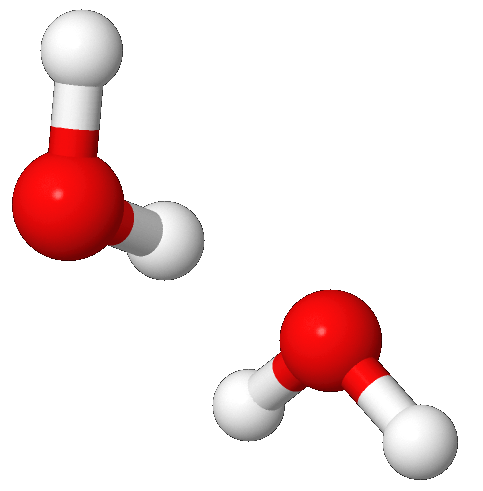
\includegraphics[width = 0.5\textwidth]{figures/h2o.png}
\caption{3D geometry of \hho\ dimer.}
\end{figure}

\begin{figure}
\centering
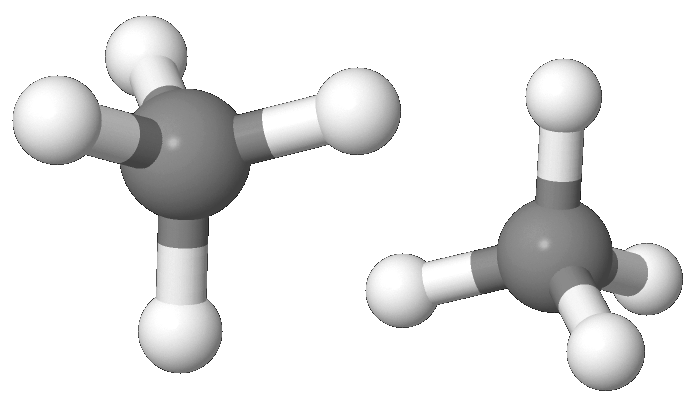
\includegraphics[width = 0.5\textwidth]{figures/ch4.png}
\caption{3D geometry of \ch\ dimer.}
\end{figure}

\begin{figure}
\centering
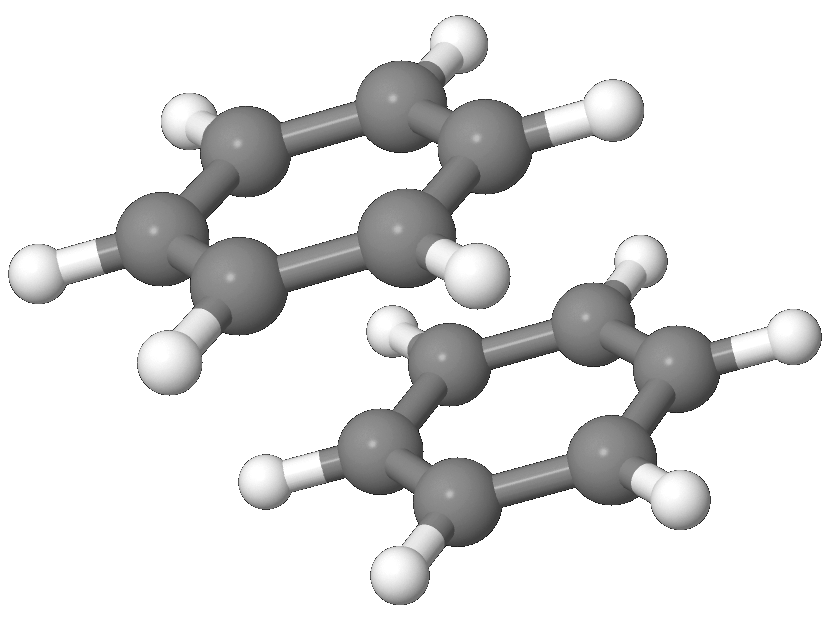
\includegraphics[width = 0.5\textwidth]{figures/benzene-parallel-displaced.png}
\caption{3D geometry of \benzpara\ dimer.}
\end{figure}

\begin{figure}
\centering
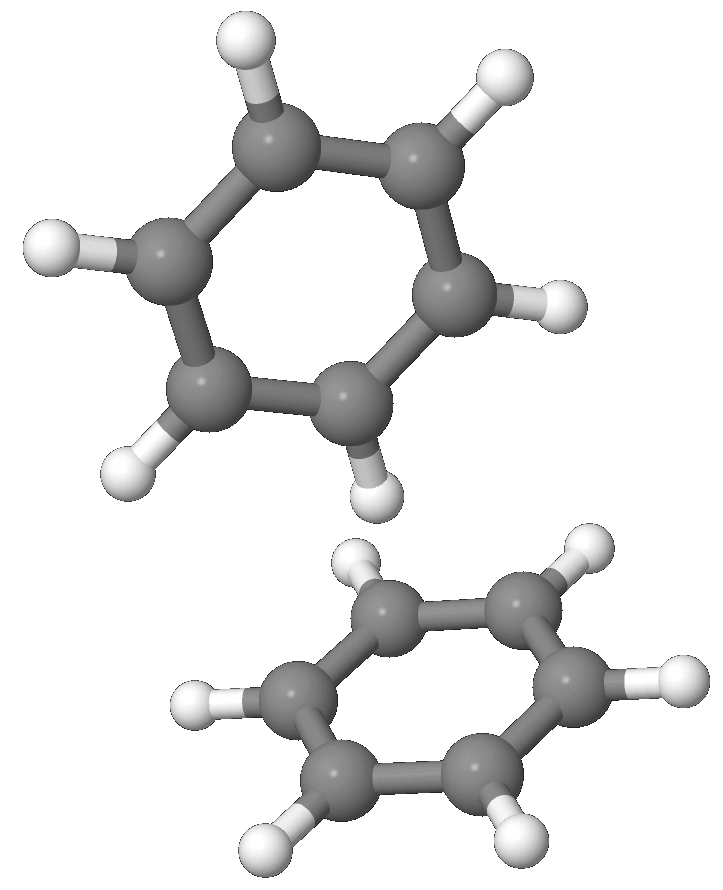
\includegraphics[width = 0.5\textwidth]{figures/benzene-T-shaped.png}
\caption{3D geometry of \benzT\ dimer.}
\end{figure}

\section{HF Calculations}

For each dimer system, the aug-cc-pVDZ basis set was used for HF and MC-MP2
calculations.

\section{MP2 Energies}



% CONCLUSIONS
\chapter{Conclusions}

\printbibliography
\addcontentsline{toc}{chapter}{Bibliography}

\end{document}
